\chapter{Projeto/Proposta de Solução}
	\label{ch:proposta}

Os conceitos revisados até este momento foram utilizados para a criação de uma proposta de solução computacional para a equipe baja Velociraptor. Revisando, a equipe tem como principal problema não conseguir obter informações que interessam a cada setor de projeto do veículo de maneira \textbf{intuitiva, simplificada, modular e com armazenamento.} Estes três conceitos são detalhados no Quadro \ref{tab:cenario} a seguir:     

\begin{table}[!htb]
	\centering
		\caption{Conceitos do cenário estudado}
		\label{tab:cenario}
	\begin{tabular}{|l|l|l|}
		\hline
		\rowcolor[HTML]{9B9B9B} 
		{\color[HTML]{000000} Conceito} & {\color[HTML]{000000} Descrição}                                                                                                                                 \\ \hline
		Intuitiva                       & \begin{tabular}[c]{@{}l@{}}Demostração dos dados com \\ gráficos e valores absolutos\end{tabular}                                                                \\ \hline
		Simplificada                    & \begin{tabular}[c]{@{}l@{}}Um sistema para aquisição \\ para todos os dados dos sensores\\ reunindo as informações de \\ todos os setores do veículo\end{tabular} \\ \hline
		Modular                    & \begin{tabular}[c]{@{}l@{}}Preparado para expansão e\\  atualização com novas \\tecnologias\end{tabular} \\ \hline
		Armazenamento                   & \begin{tabular}[c]{@{}l@{}}Armazena os dados retirados \\ dos sensores para análises \\ futuras\end{tabular}                                                     \\ \hline
	\end{tabular}
		\caption*{Fonte: Autor.}
\end{table}

\section{Objetivos}
\label{sec:objetivos}
Os objetivos que devem nortear o trabalho a fim de sanar os problemas levantados podem ser subdivididos em um objetivo geral, que é a meta final do trabalho, e objetivos específicos, que servem como diretrizes menores que quando concluídas resultaram na conclusão do trabalho como um todo.

\subsection{Objetivo Geral}

Produzir um sistema que forneça a equipe informações que irão ajudar aos setores de projeto do veículo como suspensão dianteira, suspensão traseira, freio, transmissão e eletrônica em testes de bancada, bem como fornecer dados de uso geral da equipe como média do consumo de gasolina em prova para análises posteriores. 

O sistema é dividido em duas frentes: a parte de \textbf{aquisição} dos dados, feito junto ao SCOB com base nos dados recebidos via sensores revisados na seção \ref{sec:sensores}, esta parte já existe atualmente no baja Velociraptor, porém ela foi atualizada para acompanhar os avanços do novo \textit{software}; a parte de \textbf{tratamento} dos dados é o foco deste trabalho, nesta parte os dados serão transmitidos por um módulo de transmissão de dados sem fio ZigBee e lidos por um \textit{software} que permite visualização de gráficos e mostra de valores absolutos de maior importância. A Figura \ref{fig:esquemageral} possui dois diagramas, o diagrama da Figura \ref{fig:esquemageral}\subref{fig:geralatual} traz um esquema geral que atualmente é utilizado pelo Velociraptor no seu projeto, já a Figura \ref{fig:esquemageral}\subref{fig:geralproposto} traz um esquema geral proposto para este trabalho de conclusão de curso, desde a aquisição dos dados pelos SCOBs até o tratamento dos dados nos boxes com o \textit{software}. Em ambas as figuras os balões em azul indicam os sensores, os balões em laranja indicam \textit{hardware} de controle e balões em verde indicam \textit{software}, os balões com texto em negrito indicam modificação/criação de um sistema.         

%\begin{figure}[!htb]
%	\centering
%		\caption{Diagrama com o esquema geral proposto do sistema.}
%		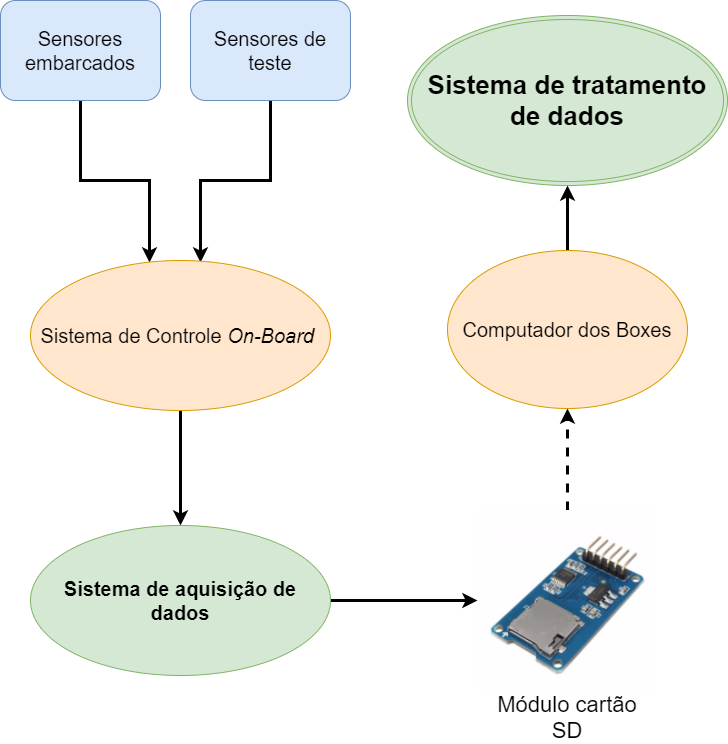
\includegraphics[scale=0.3]{geral.png} 
%		\caption*{Fonte: Autor.}
%		\label{fig:geral}
%\end{figure} 

\begin{figure}[!htb]
	\center
	\caption{Diagrama com o esquema geral do sistema atual e o esquema geral do sistema proposto.}
	\subfigure[Fonte: Autor][Esquema atual. Fonte:Autor]{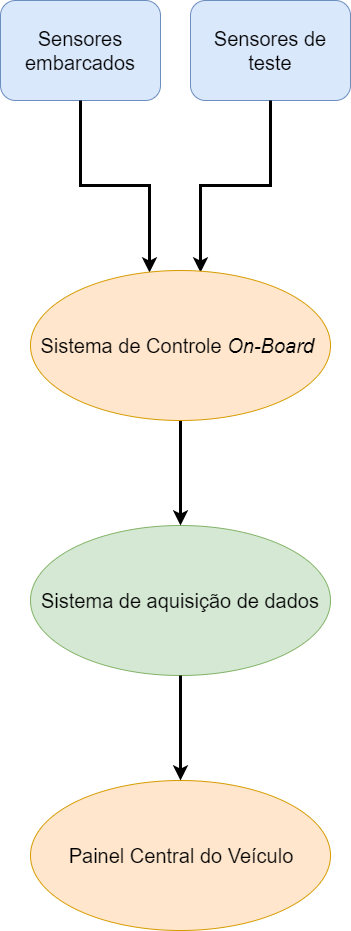
\includegraphics[scale=0.3]{geralatual}\label{fig:geralatual}}
	\qquad
	\subfigure[Fonte: Autor][Esquema proposto. Fonte:Autor]{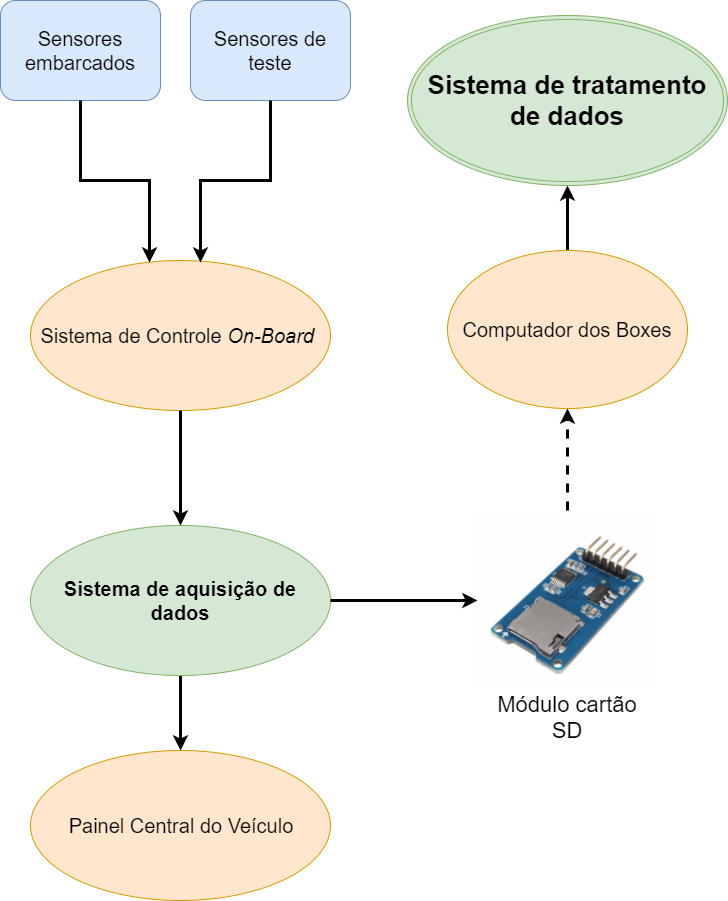
\includegraphics[scale=0.3]{geralproposto}\label{fig:geralproposto}}
	\label{fig:esquemageral}
\end{figure}


\subsection{Objetivos Específicos} 

\begin{itemize}[label={-}]
	\item O sistema deve ser independente em relação ao meio em que os dados são transportados do SCOB para os boxes, desta forma em atualizações futuras o método atual de transferência de dados pode ser substituído;
	\item O \textit{software} deve ser independente de sistema operacional;
	\item O \textit{software} deve possuir informações específicas para cada área da engenharia automobilística;
	\item O \textit{software} deve ser construído de forma a facilitar a manutenção evolutiva, preparado para chegada de novos sensores;
	\item Deve se instaurar uma cultura de utilização de plataformas de versionamento para facilitar manutenções adaptativas e manutenções corretivas.
\end{itemize}

Os objetivos específicos devem nortear a produção deste sistema. Atingindo as metas propostas se espera que o objetivo geral do projeto seja alcançado, trazendo essas informações do veículo para a equipe presente nos boxes.

\subsection{Mudanças de escopo}
O projeto teve uma mudança importante no escopo durante seu desenvolvimento e tais mudanças serão apresentadas aqui nesta seção.

Inicialmente, o projeto englobaria telemetria, a criação de um sistema de controle \textit{on-board} e a criação de um \textit{software} de tratamento dos dados provenientes do veículo. Esta ideia possuía um escopo muito amplo para ser feito por apenas uma pessoa em dois semestres, então uma nova proposta foi realizada na qual o foco seria no \textit{software} de tratamento de dados recebendo estes mesmo dados via um \textit{Secure Digital Card}, ou como é normalmente conhecido cartão SD. Este segundo escopo era mais realista em relação ao tempo de execução do projeto, levando em conta o trabalho para a criação do sistema levantando os dados necessários para uma melhor forma de demostrar as grandezas do sistema. Contudo durante reuniões do projeto 2018 do sub-sistema de eletrônica veicular do Velociraptor, foi criado um terceiro escopo de projeto em conjunto com os interesses da equipe e suas prioridades. Neste escopo, que é o atual desenvolvido e testado neste trabalho, o sistema recebe as informações dos sensores via rede sem fio utilizando um par de módulos ZigBee. Este escopo se assemelha muito ao primeiro, porém com o auxilio da equipe de eletrônica para fabricação das placas de teste, a ideia enfim se tornou viável.